% %%%%%%%%%%%%%%%%%%%%%%%%%%%%%%%%%%%%%%%%%%%%%%%%%%%%%%%%%
% Template created by Yang Ma, April-2022.
% Last update: April-2022.
% Contact: mayangluon@pitt.edu
%
% DISCLAIMER: This is not an official PITTPACC template.
% %%%%%%%%%%%%%%%%%%%%%%%%%%%%%%%%%%%%%%%%%%%%%%%%%%%%%%%%%

% ---------------------------------------
\documentclass[aspectratio=169]{beamer}
\usepackage{PITTtheme}
% ---------------------------------------

%% ===========================================
%% ===========================================
\title[short title]{\huge Main Title}
\author{First Author \& Second Author}
\institute{Food and Resource Economics Department}
\date{\today}
%% ===========================================
%% ===========================================
% Don't change this part.
\begin{document}

\begin{frame}[plain]
\Background
    \titlepage
\end{frame}

%% ===========================================
%% ===========================================
% Uncomment these lines for an automatically generated outline.
%\begin{frame}{Outline}
%  \tableofcontents
%\end{frame}
%% ===========================================
%% ===========================================
%	PRESENTATION SLIDES
%% ===========================================
%% ===========================================

%% ===========================================
%% ===========================================
\section{First Section} % Sections can be created in order to organize your presentation into discrete blocks, all sections and subsections are automatically printed in the table of contents as an overview of the talk
%% ===========================================
%% ===========================================

\subsection{Subsection Example} % A subsection can be created just before a set of slides with a common theme to further break down your presentation into chunks

%% ===========================================
%% ===========================================

\begin{frame}
\frametitle{Paragraphs of Text}
Sed iaculis dapibus gravida. Morbi sed tortor erat, nec interdum arcu. Sed id lorem lectus. Quisque viverra augue id sem ornare non aliquam nibh tristique. Aenean in ligula nisl. Nulla sed tellus ipsum. Donec vestibulum ligula non lorem vulputate fermentum accumsan neque mollis.\\~\\

Sed diam enim, sagittis nec condimentum sit amet, ullamcorper sit amet libero. Aliquam vel dui orci, a porta odio. Nullam id suscipit ipsum. Aenean lobortis commodo sem, ut commodo leo gravida vitae. Pellentesque vehicula ante iaculis arcu pretium rutrum eget sit amet purus. Integer ornare nulla quis neque ultrices lobortis. Vestibulum ultrices tincidunt libero, quis commodo erat ullamcorper id.
\end{frame}

%% ===========================================
%% ===========================================

\begin{frame}
\frametitle{Bullet Points}
\begin{itemize}
\item Lorem ipsum dolor sit amet, consectetur adipiscing elit
\item Aliquam blandit faucibus nisi, sit amet dapibus enim tempus eu
\item Nulla commodo, erat quis gravida posuere, elit lacus lobortis est, quis porttitor odio mauris at libero
\item Nam cursus est eget velit posuere pellentesque
\item Vestibulum faucibus velit a augue condimentum quis convallis nulla gravida
\end{itemize}
\end{frame}

%% ===========================================
%% ===========================================
\section{Second Section} 
%% ===========================================
%% ===========================================

\begin{frame}
\frametitle{Blocks of Highlighted Text}
\begin{block}{Regular Block}
Lorem ipsum dolor sit amet, consectetur adipiscing elit. Integer lectus nisl, ultricies in feugiat rutrum, porttitor sit amet augue. Aliquam ut tortor mauris. Sed volutpat ante purus, quis accumsan dolor.
\end{block}

\begin{exampleblock}{Example Block}
Pellentesque sed tellus purus. Class aptent taciti sociosqu ad litora torquent per conubia nostra, per inceptos himenaeos. Vestibulum quis magna at risus dictum tempor eu vitae velit.
\end{exampleblock}

\begin{alertblock}{Alert Block}
Suspendisse tincidunt sagittis gravida. Curabitur condimentum, enim sed venenatis rutrum, ipsum neque consectetur orci, sed blandit justo nisi ac lacus.
\end{alertblock}
\end{frame}

%% ===========================================
%% ===========================================

%% ===========================================
\subsection{Using columns}
%% ===========================================

%% ===========================================
%% ===========================================

\begin{frame}
\frametitle{Multiple Columns}
\begin{columns}[c] % The "c" option specifies centered vertical alignment while the "t" option is used for top vertical alignment

\column{.45\textwidth} % Left column and width
\textbf{Heading}
\begin{enumerate}
\item Statement
\item Explanation
\item Example
\end{enumerate}

\column{.5\textwidth} % Right column and width
Lorem ipsum dolor sit amet, consectetur adipiscing elit. Integer lectus nisl, ultricies in feugiat rutrum, porttitor sit amet augue. Aliquam ut tortor mauris. Sed volutpat ante purus, quis accumsan dolor.

\end{columns}
\end{frame}

%% ===========================================
%% ===========================================
\section{Third Section}
%% ===========================================
%% ===========================================
\subsection{Tables and elements}
%% ===========================================

\begin{frame}
\frametitle{Table}
\begin{table}[H] % Option 'H' means you want the table (or figure) [exactly] HERE 
\begin{tabular}{l l l} \hline
\textbf{Treatments} & \textbf{Response 1} & \textbf{Response 2}\\ \hline \hline
Treatment 1 & 0.0003262 & 0.562 \\
Treatment 2 & 0.0015681 & 0.910 \\
Treatment 3 & 0.0009271 & 0.296 \\ \hline
\end{tabular}
\caption{Table caption}
\end{table}

\end{frame}

%% ===========================================
%% ===========================================

\begin{frame}
\frametitle{Theorem}
\begin{theorem}[Arrow's impossibility]
Let $A$ be a set of outcomes, $N$ a number of voters or decision criteria. We shall denote the set of all full linear orderings of $A$ by $L(A)$.\\~\\

A (strict) social welfare function (preference aggregation rule) is a function
\begin{equation}
    F: L(A)^N \longrightarrow L(A)
\end{equation}
which aggregates voters' preferences into a single preference order on $A$.
\end{theorem}
\end{frame}

%% ===========================================
%% ===========================================

%% ===========================================
\subsection{Econometrics}
%% ===========================================

%% ===========================================
%% ===========================================

\begin{frame}
\frametitle{Common Econometrics symbols}

\begin{equation}
    \Avar (b) = \frac{\sigma^2}{n} Q^{-1} \plim \left( \frac{1}{n}X'QX \right)Q^{-1}
\end{equation}

\begin{equation}
    \sqrt{n}(b-\beta) \stackrel{d}{\longrightarrow} \N \left[0,\frac{\sigma^2}{n} Q^{-1} \plim \left( \frac{1}{n}X'\Omega X\right)Q^{-1}\right]
\end{equation}

Also, you can use the following symbols or operators:
\begin{itemize}
    \item $\E(\cdot)$, $\V(\cdot)$, $\Var(\cdot)$, $\Cov(\cdot)$, $\Corr(\cdot)$, $\tr(\cdot)$, $\rank(\cdot)$, $\N(0,1)$, $\op(\cdot)$, $\Op(\cdot)$, $\R^+$, and $\La(y,x|\beta,\sigma^2)$.
    \item $\hat \beta$, $\widehat \beta$, $\tilde \alpha$, $\widetilde \alpha$, $\bar y$, $\varepsilon \sim \chi^2_t$
\end{itemize}

\end{frame}

%% ===========================================
%% ===========================================
\section{Fourth Section}
%% ===========================================
%% ===========================================

%% ===========================================
\subsection{Figures}
%% ===========================================

%% ===========================================
%% ===========================================

\begin{frame}
\frametitle{Figure}

\centering
    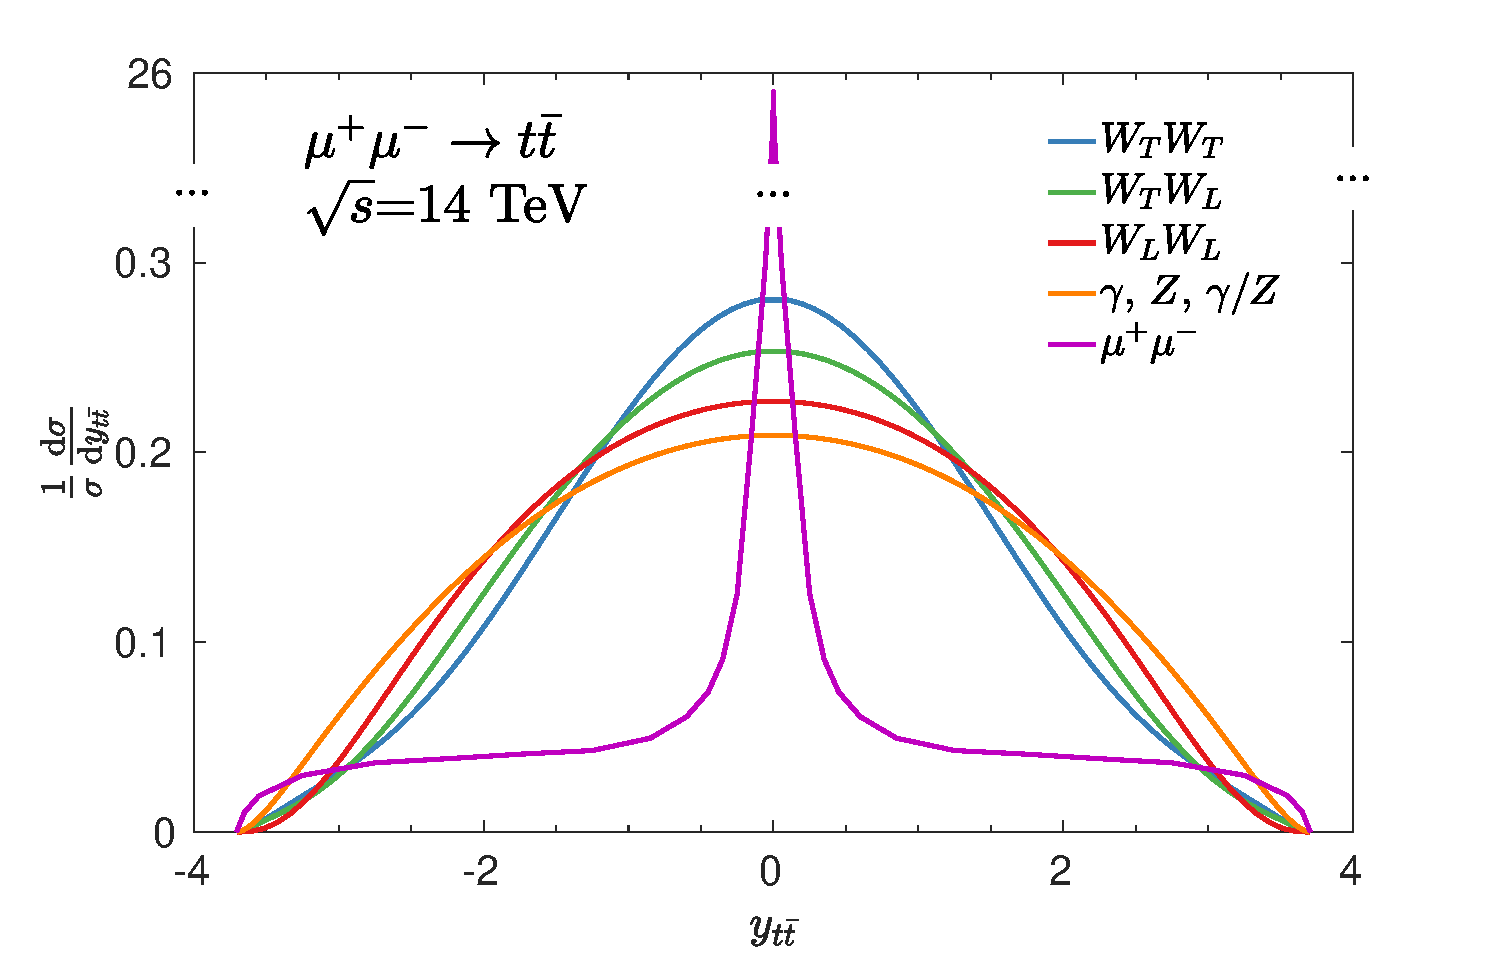
\includegraphics[width=0.48\textwidth]{fig1}
\end{frame}

%% ===========================================
%% ===========================================

\begin{frame}
\Background
\Huge{\centerline{The End}}
\end{frame}

%% ===========================================
%% ===========================================

\end{document}
